\documentclass[11pt]{scrartcl}

\usepackage[sexy]{evan}
\usepackage{pgfplots}
\pgfplotsset{compat=1.15}
\usepackage{mathrsfs}
\usetikzlibrary{arrows}
\usepackage{graphics}
\usepackage{tikz}
\usepackage{ amssymb }
\usepackage[dvipsnames]{xcolor}
\definecolor{red1}{RGB}{255, 153, 153}
\definecolor{green1}{RGB}{204, 255, 204}
\definecolor{blue1}{RGB}{204, 255, 255}
\definecolor{yellow1}{RGB}{255, 247, 160}

\definecolor{red2}{RGB}{255, 102, 102}
\definecolor{green2}{RGB}{108, 255, 108}
\definecolor{blue2}{RGB}{94, 204, 255}
\definecolor{yellow2}{RGB}{255, 250, 104}

\definecolor{red2.5}{RGB}{255,76,76}
\definecolor{green2.5}{RGB}{54, 247, 54}
\definecolor{blue2.5}{RGB}{51, 189, 255}
\definecolor{yellow2.5}{RGB}{255, 242, 52}


\definecolor{red3}{RGB}{255, 51, 51}
\definecolor{green3}{RGB}{0, 240, 0}
\definecolor{blue3}{RGB}{9, 175, 255}
\definecolor{yellow3}{RGB}{255, 234, 0}

\definecolor{red3.5}{RGB}{229, 25, 25}
\definecolor{green3.5}{RGB}{0, 194, 0}
\definecolor{blue3.5}{RGB}{4, 143, 209}
\definecolor{yellow3.5}{RGB}{255,220,0}

\definecolor{red4}{RGB}{204, 0, 0}
\definecolor{green4}{RGB}{0, 149, 0}
\definecolor{blue4}{RGB}{0, 111, 164}
\definecolor{yellow4}{RGB}{255, 206, 0}


\definecolor{noseve}{RGB}{242,242,242}

\newcommand{\camod}[1]{\frac{\ZZ}{#1 \ZZ}}
\newcommand{\modm}[1]{\text{ mod } #1}
\newcommand{\campm}[1]{\frac{\ZZ}{m\ZZ}}

\usepackage{epigraph}
\renewcommand{\epigraphsize}{\scriptsize}
\renewcommand{\epigraphwidth}{60ex}



\title {TIJM}

\author{Emmanuel Buenrostro}


\begin{document}

\maketitle


\textcolor{noseve}{No hagan esto  valorense tantito y mejor hagan OMM bien}

\section{Parte 1}
Son problemas de N1 y N2.



\subsection{C-Da el caso y ganas}
\begin{problem}[2024 N1/1]
Determine si es posible distribuir los n\'umeros del 1 al 10 en las casillas del siguiente tablero
de tal forma que cualesquiera dos n\'umeros consecutivos est\'en en casillas que no sean vecinas
(por ejemplo, 1 y 2 no deben estar en casillas vecinas, 2 y 3 no deben estar en casillas vecinas,
etc.).
\begin{center}
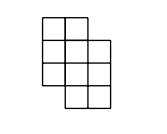
\includegraphics[scale=1]{24N11.png}
\end{center}
Aclaraci\'on. Dos casillas son vecinas si comparten un lado o un v\'ertice.
\end{problem}

\begin{problem} [2024 N1/2]
A continuaci\'on se muestra un cuadril\'atero dibujado en el papel cuadriculado. Divida al cuadril\'atero en 5 partes iguales.

\begin{center}
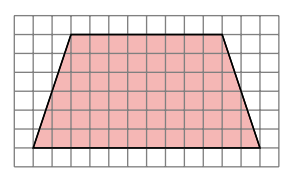
\includegraphics[scale=1]{24N12.png}
\end{center}
\end{problem}

\subsection{C- Probar que (o cuando) puedes hacer algo}
\begin{problem} [2024 N1/4 ]
Determine el mayor entero positivo $n$ para el cual existe un conjunto de $n$ enteros positivos que cumple las siguientes $n$ condiciones a la vez: 
\begin{itemize}
\item En el conjunto hay exactamente 1 m\'ultiplo de $n$.
\item En el conjunto hay exactamente 2 m\'ultiplos de $n-1$.
\item En el conjunto hay exactamente 3 m\'ultiplos de $n-2$.
\ldots
\item En el conjunto hay exactamente n m\'ultiplos de $1$.
\end{itemize}
\end{problem}


\subsection{N- Digitos}

\begin{problem} [2024 N1/3]
Un n\'umero natural de siete d\'igitos tiene la propiedad que al ser multiplicado por 4 resulta
un n\'umero que termina en 2024, es decir, es de la forma  $\ldots 2024$. Determine el menor valor
posible de la suma de los d\'igitos del n\'umero inicial.
\end{problem}
\end{document}